\documentclass[aspectratio=169,10pt]{beamer}
\usepackage[T1]{fontenc}
\usepackage{lmodern}
\usepackage{graphicx}
\usepackage{booktabs}
\usepackage{amsmath}
\usepackage{array}
\usepackage{listings}
\usepackage{xcolor}
\usepackage{tikz}

% ---- look: Computer Modern throughout, one accent colour, no chrome ---------------------------------------
\usetheme{default}
\usefonttheme{serif}
\definecolor{accent}{HTML}{2A5FB4}
\definecolor{ink}{HTML}{151515}
\definecolor{muted}{HTML}{5A5A5A}
\definecolor{soft}{HTML}{9A9A9A}
\setbeamercolor{structure}{fg=accent}
\setbeamercolor{normal text}{fg=ink}
\setbeamercolor{frametitle}{fg=ink}
\setbeamercolor{title}{fg=ink}
\setbeamercolor{subtitle}{fg=muted}
\setbeamerfont{frametitle}{series=\bfseries,size=\Large}
\setbeamerfont{title}{series=\bfseries,size=\huge}
\setbeamerfont{subtitle}{series=\itshape,size=\large}
\setbeamertemplate{navigation symbols}{}
\setbeamertemplate{itemize items}{\color{accent}\raisebox{0.15ex}{\rule{0.5ex}{0.5ex}}}
\setbeamertemplate{frametitle}{\vspace{0.9em}\insertframetitle\par\vspace{-0.25em}
  {\color{soft}\rule{0.2\textwidth}{0.5pt}}\vspace{0.1em}}
\setbeamertemplate{footline}{%
  \hspace*{1.2em}{\color{soft}\scriptsize Synthetix Alpha}\hfill
  {\color{soft}\scriptsize\insertframenumber\,/\,\inserttotalframenumber}\hspace*{1.2em}\vspace{0.7em}}
\setlength{\leftmargini}{1.1em}
\setbeamersize{text margin left=1.6em,text margin right=1.6em}
\lstset{basicstyle=\ttfamily\scriptsize\color{ink},columns=fullflexible,keepspaces=true,frame=none,xleftmargin=0pt}
\graphicspath{{img/}}
\newcommand{\muted}[1]{{\color{muted}#1}}
\newcolumntype{L}[1]{>{\raggedright\arraybackslash}p{#1}}

\title{Synthetix Alpha}
\subtitle{An autonomous, risk-gated trading agent on Alpaca}
\author{Alan Smith\inst{1} \and Ciprian Mitoceanu\inst{2} \and Dhairya Sindhwani\inst{3}}
\institute{\inst{1}King's College London \quad \inst{2}University of Bucharest \quad \inst{3}Imperial College London}
\date{\muted{Alpaca AI Trading Agents Hackathon \textperiodcentered\ September 2026}}

\begin{document}

% ---- 1 title ------------------------------------------------------------------------------------------------
{\setbeamertemplate{footline}{}
\begin{frame}[plain]
  \vspace{1.0cm}
  \titlepage
  \vfill
  \begin{center}
    
\includegraphics[height=0.85cm]{alpaca.png}\hspace{1.2cm}
    
\includegraphics[height=0.85cm]{featherless.png}\hspace{1.2cm}
    
\includegraphics[height=0.85cm]{hostinger.png}
  \end{center}
  \vspace{0.5cm}
\end{frame}}

% ---- 2 cover ------------------------------------------------------------------------------------------------
{\setbeamertemplate{footline}{}
\begin{frame}[plain]
  \begin{tikzpicture}[remember picture,overlay]
    \node at (current page.center) {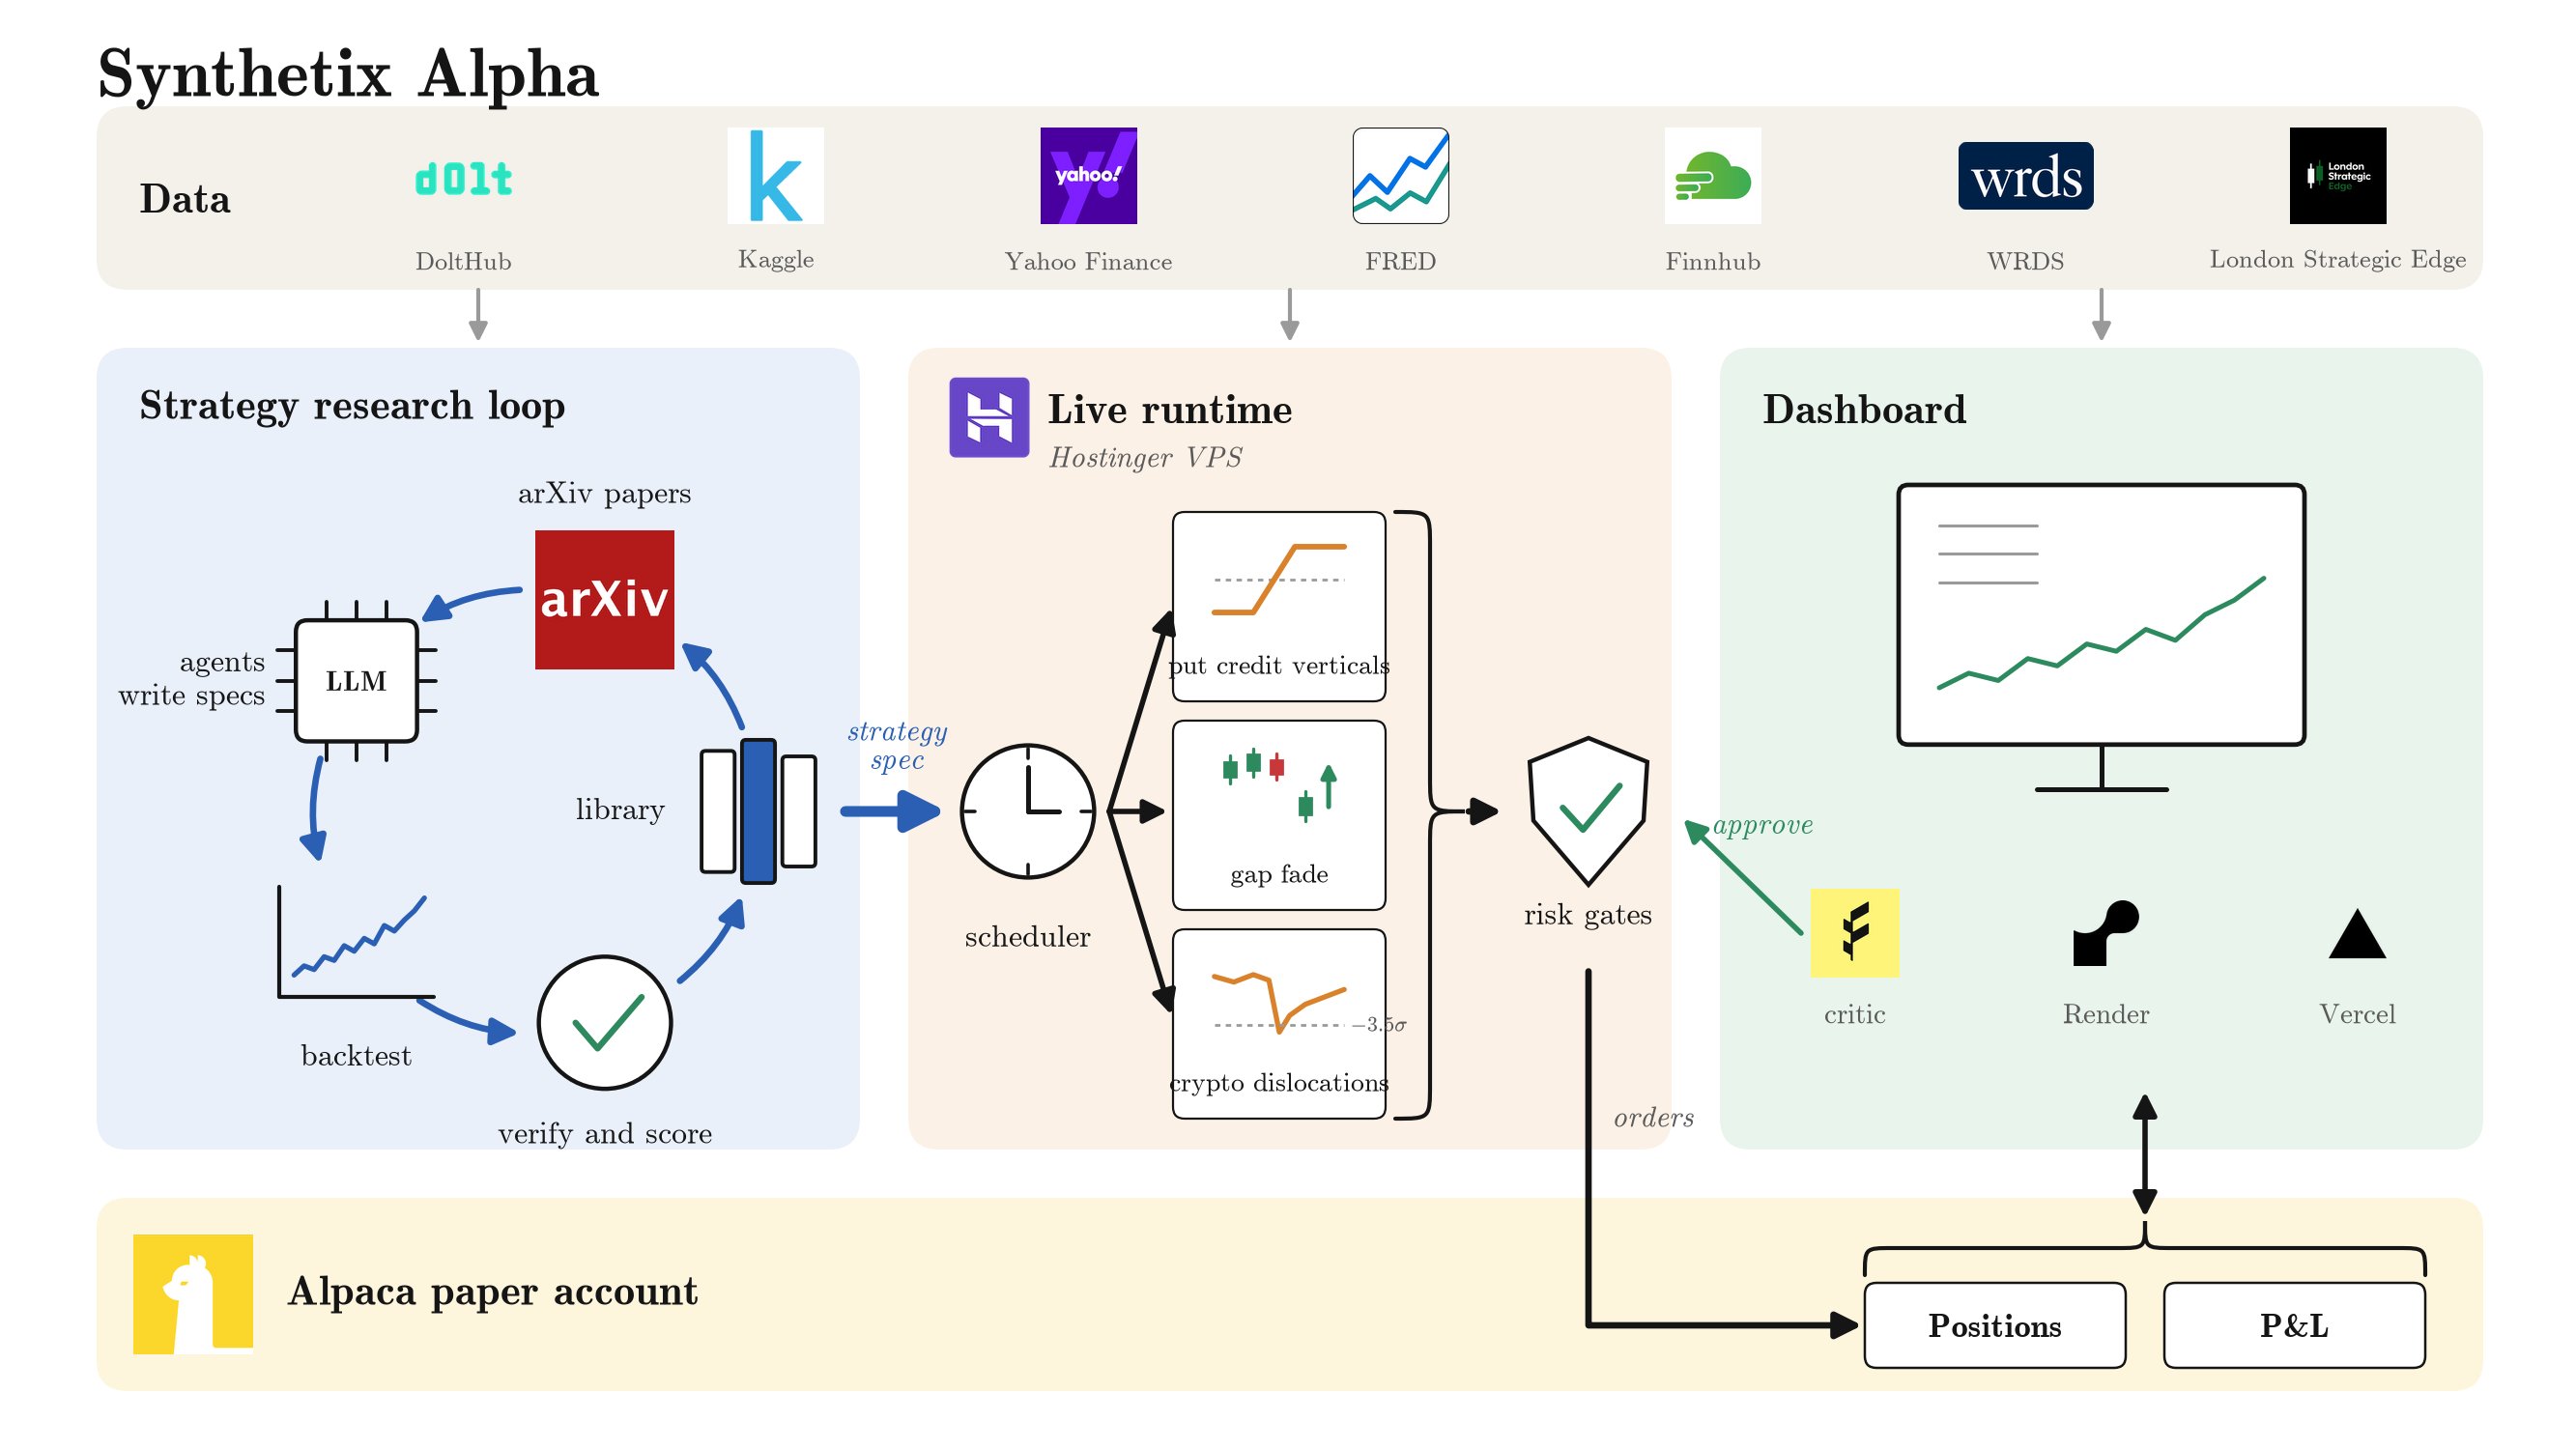
\includegraphics[width=\paperwidth]{cover.png}};
  \end{tikzpicture}
\end{frame}}

% ---- 3 the rule -----------------------------------------------------------------------------------------------
\begin{frame}{One hard rule}
  \vspace{0.3em}
  {\Large LLM agents research. \quad A deterministic runtime trades.}
  \vspace{0.9em}
  \begin{columns}[T]
    \begin{column}{0.48\textwidth}
      \structure{\textbf{Where an LLM helps}}
      \begin{itemize}
        \item reading quant-finance papers and turning their ideas into testable strategies
        \item writing strategy specs, not code, so every idea runs through the same backtester
        \item reviewing a candidate trade the way a risk officer would
      \end{itemize}
    \end{column}
    \begin{column}{0.48\textwidth}
      \structure{\textbf{Where it must not be}}
      \begin{itemize}
        \item the order path: every session runs the same rules, on a schedule, with no model call
        \item sizing and risk: fixed limits read from a config file, not a prompt
        \item the broker: the LLM never holds a key and never sees the CLI
      \end{itemize}
    \end{column}
  \end{columns}
  \vspace{0.9em}
  \muted{Live behaviour is reproducible line by line. The research is where the model earns its place.}
\end{frame}

% ---- 4 data -----------------------------------------------------------------------------------------------
\begin{frame}{Data}
  \centering
  
\includegraphics[width=0.94\textwidth]{crop_data.png}
  \vspace{0.5em}
  \footnotesize
  \begin{tabular}{@{}L{3.1cm}L{6.2cm}L{4.4cm}@{}}
    \toprule
    source & what it provides & used for \\
    \midrule
    DoltHub & IV surfaces and HV/IV history, 1,500 names, 2019--2026 & live screen, out-of-sample backtests \\
    Kaggle & end-of-day option chains with greeks, 2016--2023 & in-sample backtests \\
    Yahoo Finance & earnings dates, split history & earnings gate, split adjustment \\
    FRED & VIX, VXN, VXV, NFCI, macro series & volatility features, critic context \\
    Finnhub & news, analyst and insider sentiment & critic context \\
    WRDS & OptionMetrics and CRSP & spread and factor validation \\
    London Strategic Edge & option chains, session bars & feed reconciliation \\
    arXiv & q-fin papers & the research loop \\
    Alpaca & chains, bars to one minute, crypto; paper trading & everything live \\
    \bottomrule
  \end{tabular}
\end{frame}

% ---- 5 research loop ----------------------------------------------------------------------------------------
\begin{frame}{Strategy research loop}
  \begin{columns}[T]
    \begin{column}{0.4\textwidth}
      \vspace{0.3em}
      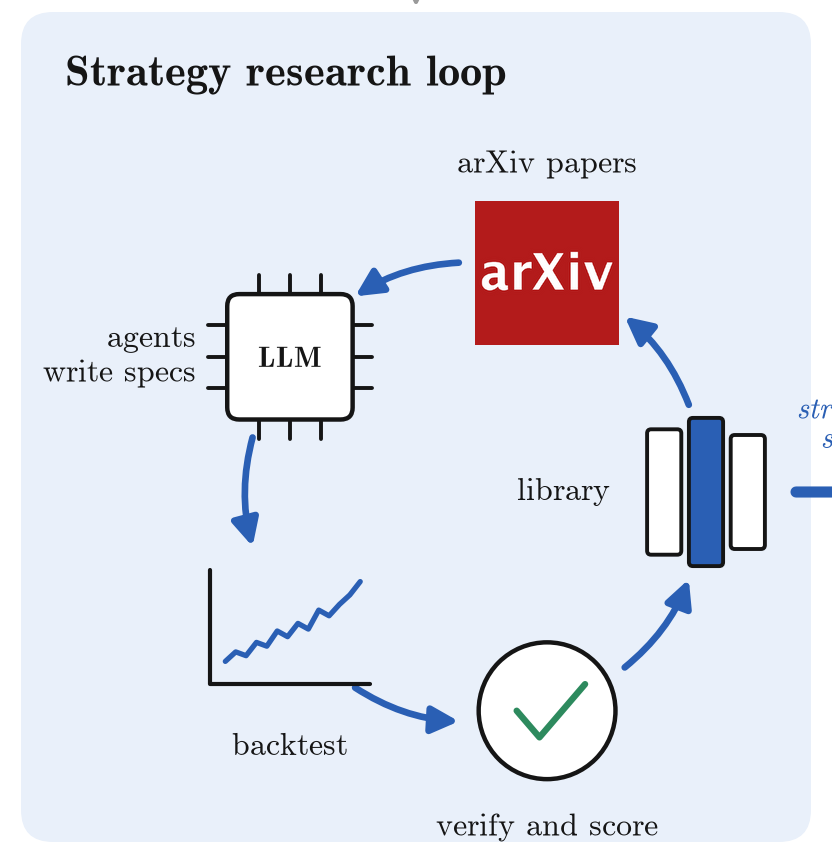
\includegraphics[width=\textwidth]{crop_research.png}
    \end{column}
    \begin{column}{0.57\textwidth}
      \vspace{0.3em}
      \begin{itemize}
        \item \textbf{arXiv intake.} q-fin categories on a paced API, keyword relevance, PDFs into an
              append-only library.
        \item \textbf{Agents write specs.} One agent per paper writes candidate strategies in a JSON DSL. The brief
              carries what is already known, forbids tuning on the backtest, and treats gains under 0.54 Sharpe as noise.
        \item \textbf{Backtest.} Real chains replayed day by day.
        \item \textbf{Verify and score.} Robustness first; unseen vendor and unseen underlying; fragility sweep.
        \item \textbf{Library.} Append-only progress log; promotion to live is a human step.
      \end{itemize}
      \vspace{0.3em}
      \muted{140+ candidates evaluated; 29 papers in the library.}
    \end{column}
  \end{columns}
\end{frame}

% ---- 6 spec + engine ----------------------------------------------------------------------------------------
\begin{frame}[fragile]{The spec DSL and the backtest engine}
  \begin{columns}[T]
    \begin{column}{0.47\textwidth}
      \structure{\textbf{A strategy is data, not code}}
      \vspace{0.4em}
\begin{lstlisting}
{ "name": "put_vertical_ivrv",
  "legs": [
    {"type": "put", "side": "short",
     "delta": 0.20},
    {"type": "put", "side": "long",
     "delta": 0.10} ],
  "underlyings": ["SPY", "QQQ"],
  "dte_target": 65,
  "dte_min": 40, "dte_max": 90,
  "signal": {
    "iv_rv_ratio":  [1.27, null],
    "vix_rv_ratio": [1.40, null] },
  "profit_target": 0.65,
  "stop_loss": 2.0, "dte_exit": 21,
  "risk_fraction": 0.03,
  "sizing": "max_loss",
  "min_volume": 25, "min_credit": 0.05 }
\end{lstlisting}
    \end{column}
    \begin{column}{0.5\textwidth}
      \structure{\textbf{What the engine does with it}}
      \begin{itemize}
        \item picks legs by delta, moneyness or width on the expiry nearest the DTE target
        \item fills at mid $\pm$ half the spread, \$0.65 per contract and leg; marks at mid; settles at intrinsic
        \item refuses contracts with no same-day volume: a mid in a contract that never traded is a quote, not a fill
        \item carries positions through stock splits the way the OCC does
        \item sizes by max loss on the payoff grid; exits on profit target, stop, DTE or hold limit
        \item 22 trailing-only features: IV surface, realised vol, VIX family, earnings, FOMC, technicals
      \end{itemize}
    \end{column}
  \end{columns}
\end{frame}

% ---- 7 verify -----------------------------------------------------------------------------------------------
\begin{frame}{Verify and score}
  \vspace{0.2em}
  \small
  \[
    \text{score} = \tfrac12\,\bar S + \tfrac12\,S_{\min} + 2\cdot\text{worst year} + 3\cdot\max(\text{maxDD},-1)
                   + (\text{positive years} - 1)
  \]
  \centering\muted{$-9$ under 40 trades, so a thin sample can never win}
  \vspace{0.6em}
  \begin{columns}[T]
    \begin{column}{0.5\textwidth}
      \begin{itemize}
        \item \textbf{Unseen vendor.} Fitted on Kaggle chains, re-run on DoltHub surfaces 2019--2026.
        \item \textbf{Unseen underlying.} AAPL was never used to fit the index rule.
        \item \textbf{Fragility sweep.} Every parameter perturbed one at a time; the median perturbed score is part
              of the objective from generation 3 on.
        \item \textbf{Concentration.} The top five trades must not carry the P\&L.
      \end{itemize}
    \end{column}
    \begin{column}{0.46\textwidth}
      \begin{tabular}{@{}lrr@{}}
        \toprule
        put credit vertical & Sharpe & trades \\
        \midrule
        in sample, Kaggle SPY+QQQ & 0.92 & 102 \\
        DoltHub SPY 2019--2026 & 0.65 & 148 \\
        AAPL 2016--2023, unseen & 0.49 & 184 \\
        \bottomrule
      \end{tabular}
      \vspace{0.5em}

      \muted{The number we plan around is the out-of-sample one. The in-sample gap closed once the liquidity floor
      was added: the filter removed illusion, not edge.}
    \end{column}
  \end{columns}
\end{frame}

% ---- 8 evolution I ----------------------------------------------------------------------------------------
\begin{frame}{Strategy evolution: the search}
  \footnotesize
  \begin{tabular}{@{}cL{4.1cm}rrL{6.6cm}@{}}
    \toprule
    gen & strategy & Sharpe & score & what changed \\
    \midrule
    0 & put spread, IV-rank gate & $-0.13$ & $-1.18$ & hand-written baseline \\
    0 & put spread, IV/RV gate & 0.73 & 0.40 & conditional premium selling \\
    0 & diagonal put credit & 0.85 & 0.75 & generation winner, only 49 trades \\
    2 & put spread, IV/RV gate & 1.01 & 0.98 & winner, but $\pm10$ DTE collapses it to 0.28 / 0.07 \\
    3 & \textbf{put vertical, 65 DTE} & 1.14 & 1.09 & re-centred onto the 55--70 DTE plateau; fragility fixed \\
    4 & put vertical, double gate & 1.15 & 1.11 & VIX or VXN must confirm the chain-derived gate \\
    4 & \muted{same, liquidity floor} & \muted{0.92} & \muted{0.52} & \muted{25 contracts of same-day volume; 9.8\% of earlier fills had none} \\
    5 & single-name vertical, AAPL & 0.90 & 0.84 & earnings filter: no announcement within 30 days \\
    7--8 & three-sleeve portfolio & 0.97 & 0.91 & index, single-name and bear-call sleeves, equal weight \\
    \bottomrule
  \end{tabular}
  \vspace{0.7em}
  \normalsize
  \begin{itemize}
    \item 8 strategy angles, 2 seeds each; three generations of mutation and crossover on the top five; agents ran
          concurrently and each verified its own candidate.
    \item Corrections are logged even when the score falls. A number no longer believed does not stay the headline.
  \end{itemize}
\end{frame}

% ---- 9 evolution II ---------------------------------------------------------------------------------------
\begin{frame}{Strategy evolution: what survived}
  \begin{columns}[T]
    \begin{column}{0.48\textwidth}
      \structure{\textbf{Kept}}
      \begin{itemize}
        \item selling put spreads only when implied vol is rich to realised; unconditional selling loses to costs
        \item 65 DTE, on the plateau rather than the edge of the 35--45 DTE hole; 20/10-delta wings; 65\% profit
              target; exit at 21 DTE
        \item an earnings blackout for single names: AAPL score $-0.15 \to +0.84$
        \item equal weights across sleeves: every optimised weighting won in sample and lost out of sample
      \end{itemize}
    \end{column}
    \begin{column}{0.48\textwidth}
      \structure{\textbf{Tried and dropped}}
      \begin{itemize}
        \item long-vol structures: straddles, strangles and calendars carry negatively
        \item 60-day condors; 4-DTE technical-signal spreads (AAPL 0.80, QQQ $-0.14$)
        \item ``skip the crisis'': dropping high-VIX days cut the score 1.09 $\to$ 0.76; panic is when the premium
              is richest
        \item the diagonal, once the vertical moved to 65 DTE; five paper ideas and a FOMC event rule, each
              rejected out of sample
      \end{itemize}
    \end{column}
  \end{columns}
  \vspace{0.7em}
  \muted{Checked on OptionMetrics with overlap-corrected errors, the gate's advantage sits inside the noise. It stays
  as a filter; the expectation we carry is the out-of-sample Sharpe.}
\end{frame}

% ---- 10 options rule in production ------------------------------------------------------------------------
\begin{frame}{The options sleeve}
  \begin{columns}[T]
    \begin{column}{0.4\textwidth}
      \vspace{0.3em}
      \begin{itemize}
        \item sell the 20-delta put, buy the 10-delta put, about 65 days out
        \item enter when IV/RV $\geq 1.27$ and VIX/RV $\geq 1.4$
        \item exit at 65\% of the credit, a 2$\times$ stop, or 21 DTE
        \item 3\% of equity at risk per position, 12 slots, daily entry
        \item 25 contracts of same-day volume; credit at least 5\% of max loss
      \end{itemize}
      \vspace{0.4em}
      \muted{Backtest 2020--2022 on SPY and QQQ: 102 trades, Sharpe 0.92, max drawdown 2.0\%.}
    \end{column}
    \begin{column}{0.58\textwidth}
      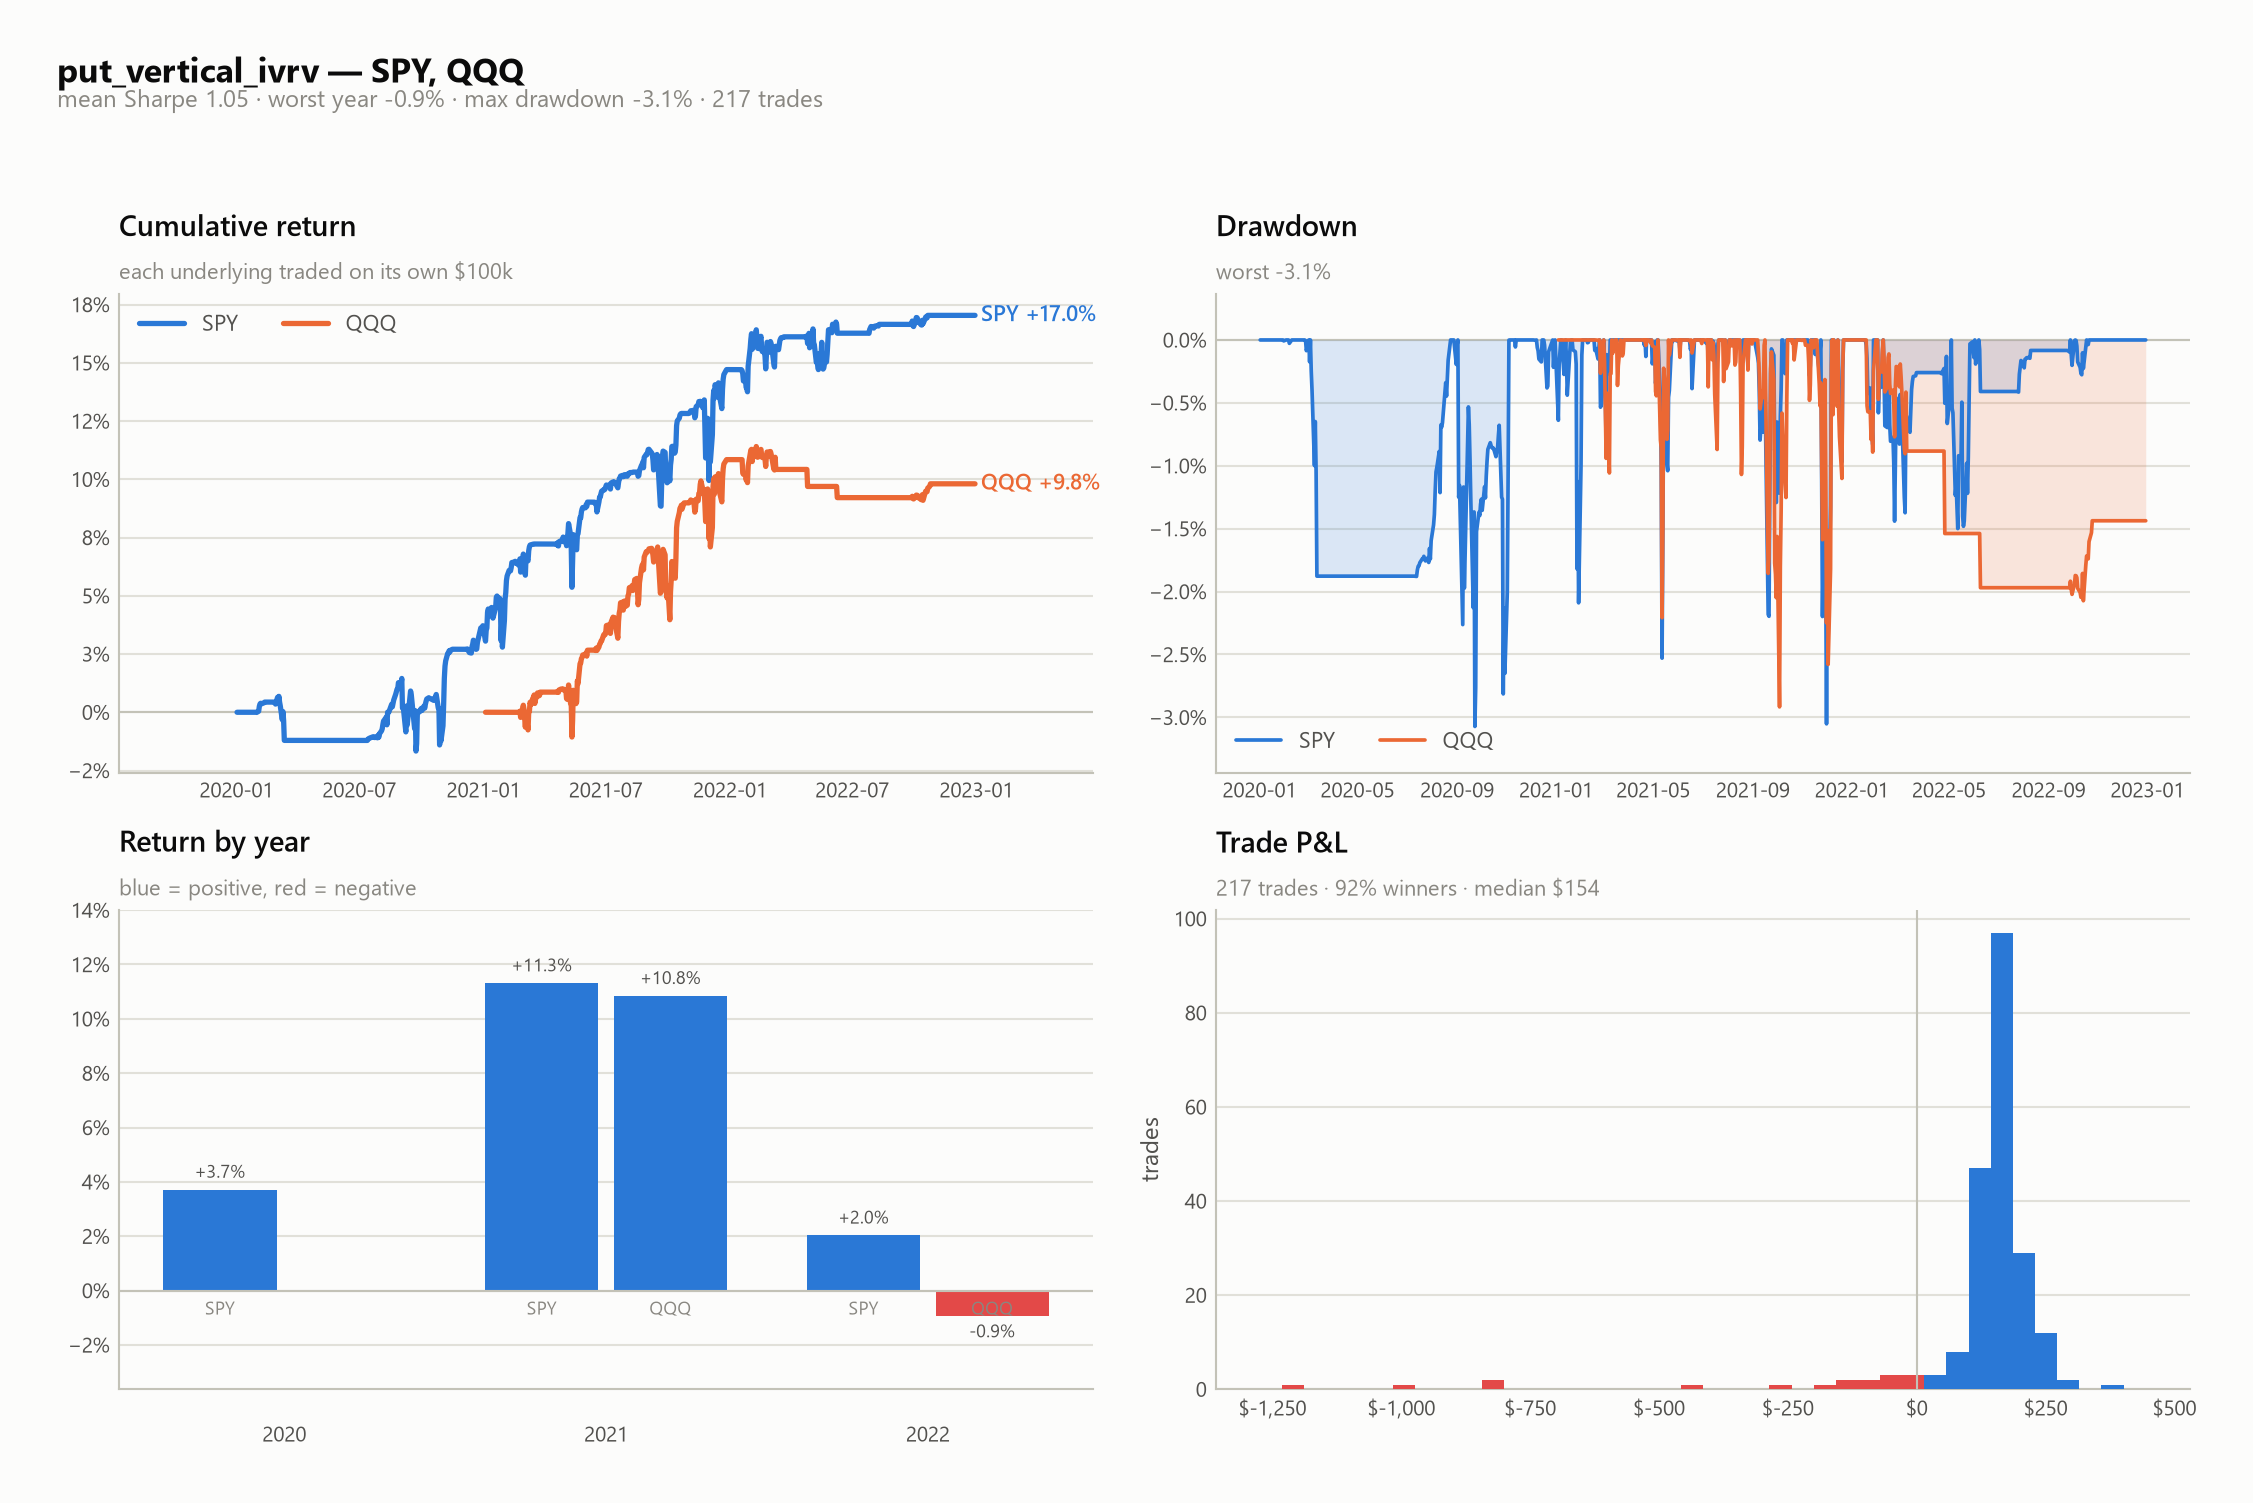
\includegraphics[width=\textwidth]{put_vertical_ivrv_performance.png}
    \end{column}
  \end{columns}
\end{frame}

% ---- 11 intraday research -----------------------------------------------------------------------------------
\begin{frame}{An intraday sleeve, and what minute bars showed}
  \begin{columns}[T]
    \begin{column}{0.48\textwidth}
      \structure{\textbf{The gap fade}}
      \begin{itemize}
        \item 198 large caps; rank the overnight gap by 20-day volatility; buy the ten most negative at the open,
              flat by the close
        \item daily-bar backtest, five years: 4.6\,bp a day net of measured spreads, Sharpe 0.65
        \item defects found and masked on the way: opens copied from closes, a busted opening auction, unadjusted
              splits, spin-off mismatches between feeds
      \end{itemize}
    \end{column}
    \begin{column}{0.48\textwidth}
      \structure{\textbf{Re-measured from the fill}}
      \vspace{0.2em}
      \small
      \begin{tabular}{@{}lrr@{}}
        \toprule
        leg, Alpaca 1-min bars & bp/day & $t$ \\
        \midrule
        official open $\to$ 09:31 print & $+5.0$ & 7.6 \\
        09:31 $\to$ 10:00 & $+0.1$ & 0.1 \\
        10:00 $\to$ 15:50 & $+1.1$ & 0.4 \\
        select on an independent open & $+0.3$ & 0.5 \\
        \bottomrule
      \end{tabular}
      \vspace{0.4em}

      The whole backtested edge sits between the auction print and the first trade after it, a price no market
      order can get. Selecting on a different noisy open removes it.
    \end{column}
  \end{columns}
  \vspace{0.5em}
  \muted{The loop re-measured its own strategy from the price an order actually meets and reported the answer.}
\end{frame}

% ---- 12 live runtime ----------------------------------------------------------------------------------------
\begin{frame}{Live runtime}
  \begin{columns}[T]
    \begin{column}{0.38\textwidth}
      \vspace{0.3em}
      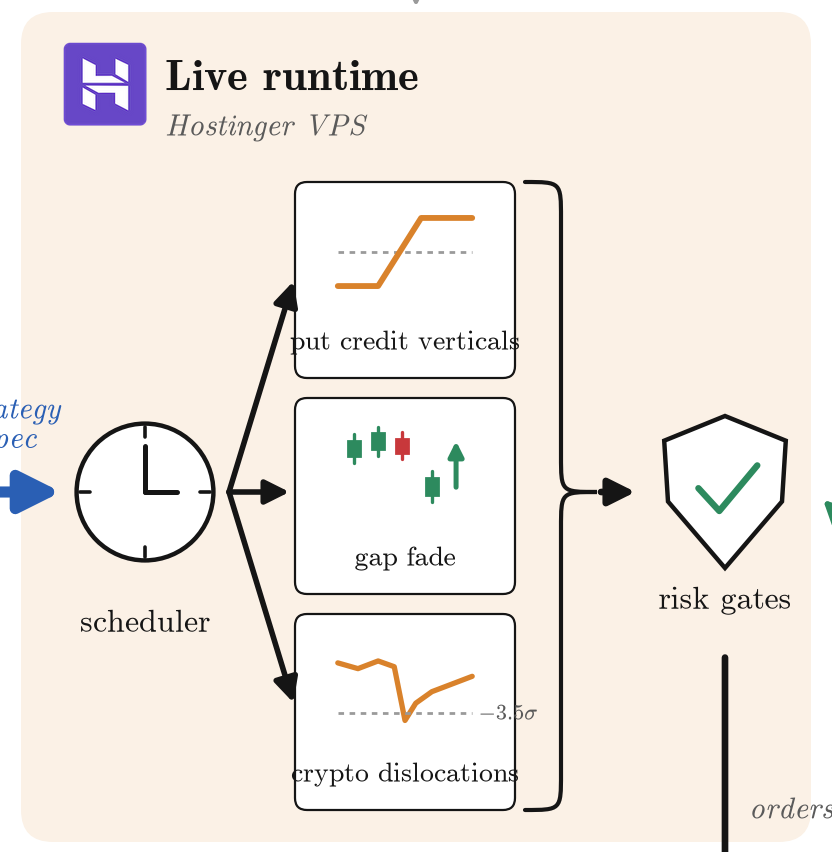
\includegraphics[width=\textwidth]{crop_runtime.png}
    \end{column}
    \begin{column}{0.59\textwidth}
      \vspace{0.3em}
      \begin{itemize}
        \item \textbf{Scheduler} on a Hostinger VPS: 09:31 enter, 09:45 top-up, 15:50 and 15:56 flatten (ET). State is
              marked before firing, so a crash never retries; a cron watchdog restarts it within five minutes.
        \item \textbf{A clean subprocess per fire}, with its own credentials, dry run unless told to execute.
        \item \textbf{Three sleeves}: put credit verticals; the equity gap fade at 150\% of NAV, flat by the close;
              crypto dislocations, a 24-hour move below $-3.5\sigma$ held 48 hours, at most three open.
        \item \textbf{Windows}: entries 09:31--10:30, flattening 15:30--15:58, weekends refused.
        \item \textbf{Alpaca CLI} for every account read and order; the SDK only for market data.
      \end{itemize}
    \end{column}
  \end{columns}
\end{frame}

% ---- 13 risk gates ---------------------------------------------------------------------------------------
\begin{frame}{Risk gates and execution}
  \small
  \begin{columns}[T]
    \begin{column}{0.48\textwidth}
      \structure{\textbf{Before an order exists} \muted{(governance.yaml)}}
      \begin{itemize}
        \item NAV must be positive; halt at 20\% total or 5\% daily drawdown
        \item leverage 1$\times$; 10\% of NAV per name; 12 open positions
        \item defined-risk structures only; 3\% of equity at risk per position
        \item screen: IV/RV in 1.25--2, \$20M average daily volume, chain spread under 10\%, no earnings within
              30 days
        \item crossing check: the credit at bid and ask must clear 60\% of the mid credit
        \item corporate-action guard: a large cap does not open 25\% lower on anything a fade can trade
      \end{itemize}
    \end{column}
    \begin{column}{0.48\textwidth}
      \structure{\textbf{Once it does}}
      \begin{itemize}
        \item multi-leg limit orders, up to four legs, day time in force
        \item client order id $=$ hash of the legs and the date; the same spread on the same day is the same id,
              checked in a local ledger and against the broker's open, closed and all orders
        \item status is never ``filled'' unless Alpaca said so
        \item exits sized to the actual fill; flattening covers only what is held and skips anything resting
        \item a paper-only assertion refuses to run if live trading is switched on anywhere in the environment
      \end{itemize}
    \end{column}
  \end{columns}
\end{frame}

% ---- 14 dashboard ------------------------------------------------------------------------------------------
\begin{frame}{Operator dashboard and the Featherless critic}
  \begin{columns}[T]
    \begin{column}{0.38\textwidth}
      \vspace{0.3em}
      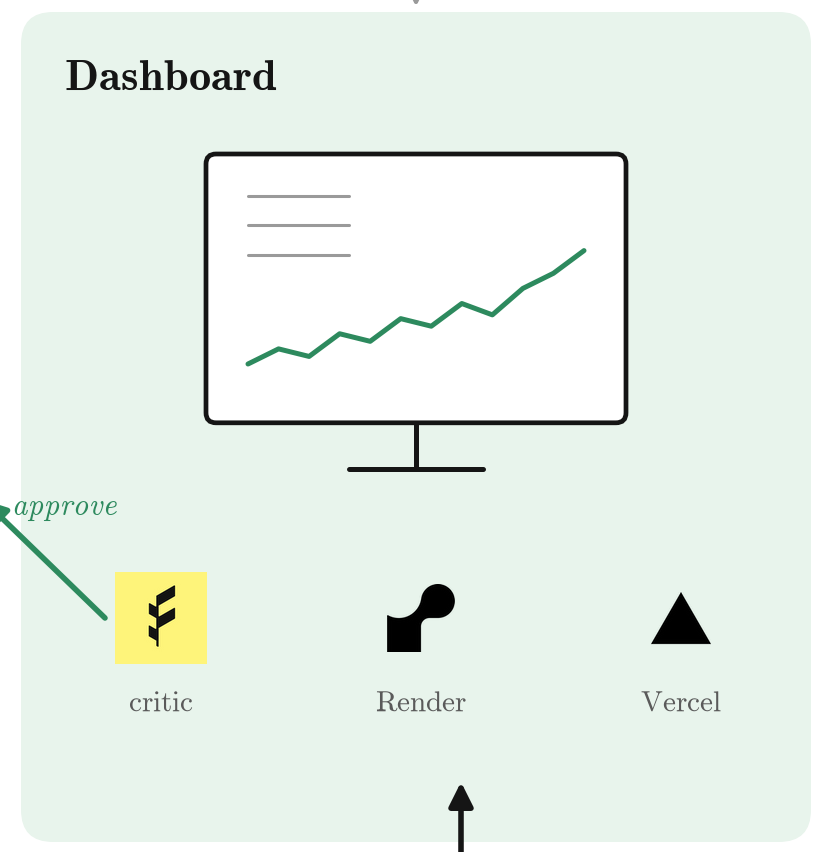
\includegraphics[width=\textwidth]{crop_dashboard.png}
    \end{column}
    \begin{column}{0.59\textwidth}
      \vspace{0.3em}
      \begin{itemize}
        \item \textbf{FastAPI} adapter in a Docker image with the Alpaca CLI, on Render; \textbf{Next.js} command
              centre on Vercel: pipeline trace, opportunities, positions, execution ledger, research view.
        \item \textbf{Pipeline}: screen $\to$ gather (Finnhub, FRED) $\to$ critique $\to$ form $\to$ risk $\to$
              operator approval $\to$ paper execution.
        \item \textbf{The critic} is a Featherless-hosted model prompted as a risk officer: approve or reject with a
              confidence and a size multiplier; reject on imminent earnings, a deep curve inversion with tightening
              conditions, or adverse headlines.
        \item \textbf{Advisory by construction}: every approval re-runs the deterministic risk gate on that single
              order, and the operator confirms in two steps.
      \end{itemize}
    \end{column}
  \end{columns}
\end{frame}

% ---- 15 result ------------------------------------------------------------------------------------------------
\begin{frame}{Paper trading, 31 August to 3 September}
  \begin{columns}[T]
    \begin{column}{0.68\textwidth}
      \vspace{0.3em}
      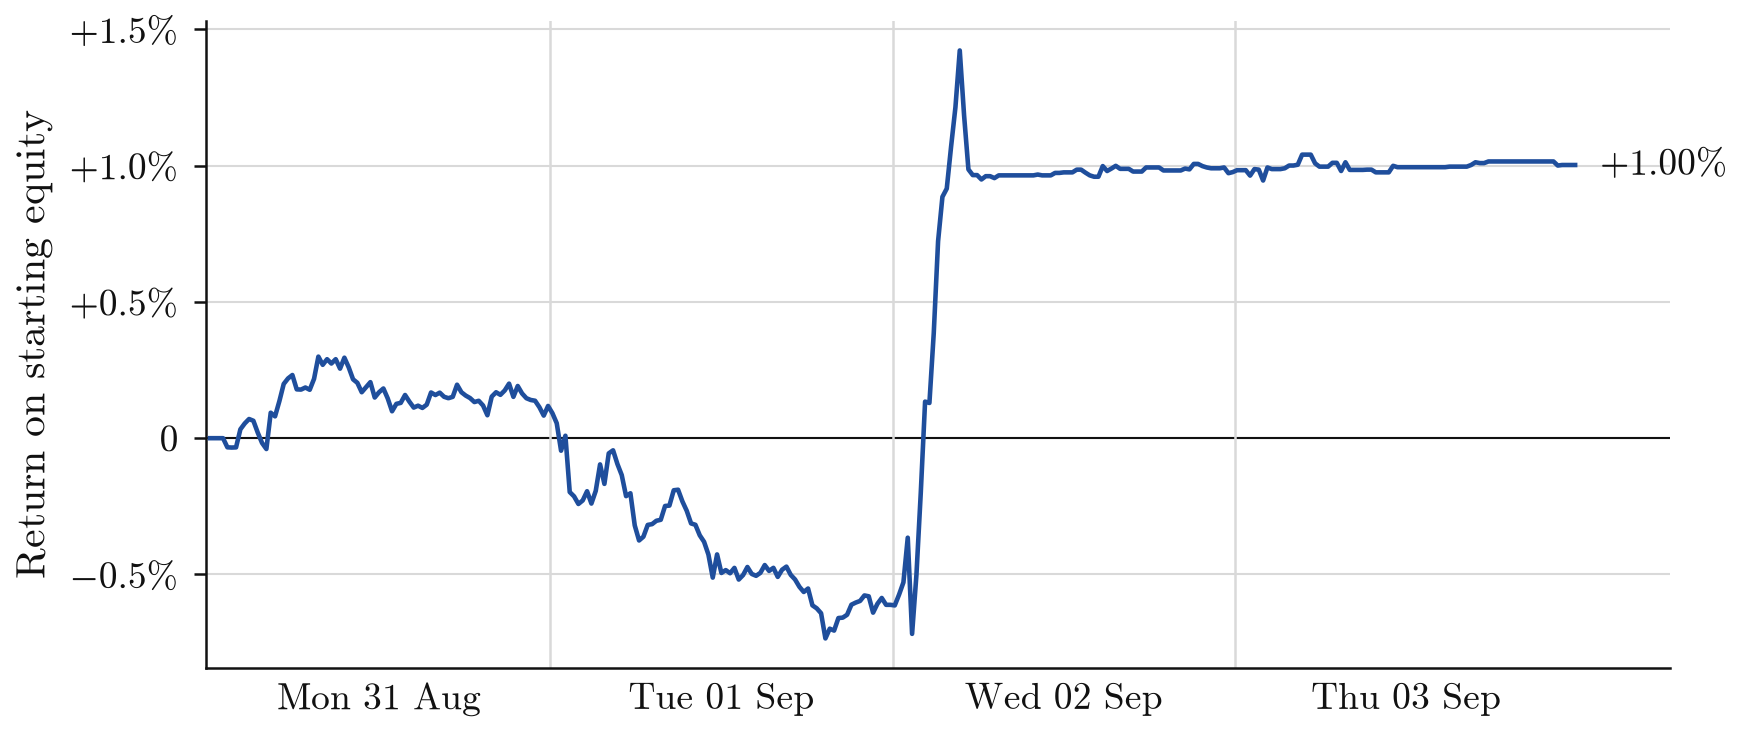
\includegraphics[width=\textwidth]{paper_pnl.png}
    \end{column}
    \begin{column}{0.3\textwidth}
      \vspace{0.8em}
      \begin{itemize}
        \item four sessions, 5-minute marks, regular hours
        \item every scheduled fire on time: entries, top-ups, flattens
        \item an options spread filled and carried through the week
        \item every gate, order id and fill reconciled against the broker
      \end{itemize}
    \end{column}
  \end{columns}
\end{frame}

% ---- 16 next --------------------------------------------------------------------------------------------------
\begin{frame}{What we would do next}
  \begin{itemize}
    \item \textbf{Rank on pre-market quotes and buy the auction.} The only place the gap fade's edge exists is the
          opening print itself, which needs market-on-open orders and a ranking that never sees the print.
    \item \textbf{Put the critic in the loop with a live key} and measure its approvals against realised outcomes,
          the way every other component was measured.
    \item \textbf{Larger option capacity.} The rule runs about one contract a trade; the same Sharpe scales to
          twenty times the return with daily entry and more slots.
    \item \textbf{Keep the research loop running.} It is append-only, it logs its corrections, and it has already
          caught its own best-looking result.
  \end{itemize}
  \vspace{1.5em}
  \begin{center}
    \muted{github.com/alan-d-smith/synthetix-alpha}
  \end{center}
\end{frame}

\end{document}
